\chapter{Backend} \label{cap:backend}

\section{Organization} \label{sec:be_organization}

The backend is a Spring Boot application written in Kotlin, structured as a set of
loosely coupled Gradle modules. Each module has a well-defined responsibility and
depends only on modules below it in the hierarchy, ensuring that business logic
remains isolated from infrastructure concerns, following principles commonly associated
with Clean Architecture~\cite{martin2017clean}. Figure~\ref{fig:backend_layers}
illustrates the module organization and the dependency relationships between them.

\begin{figure}[H]
      \begin{center}
            \resizebox{\textwidth}{!}{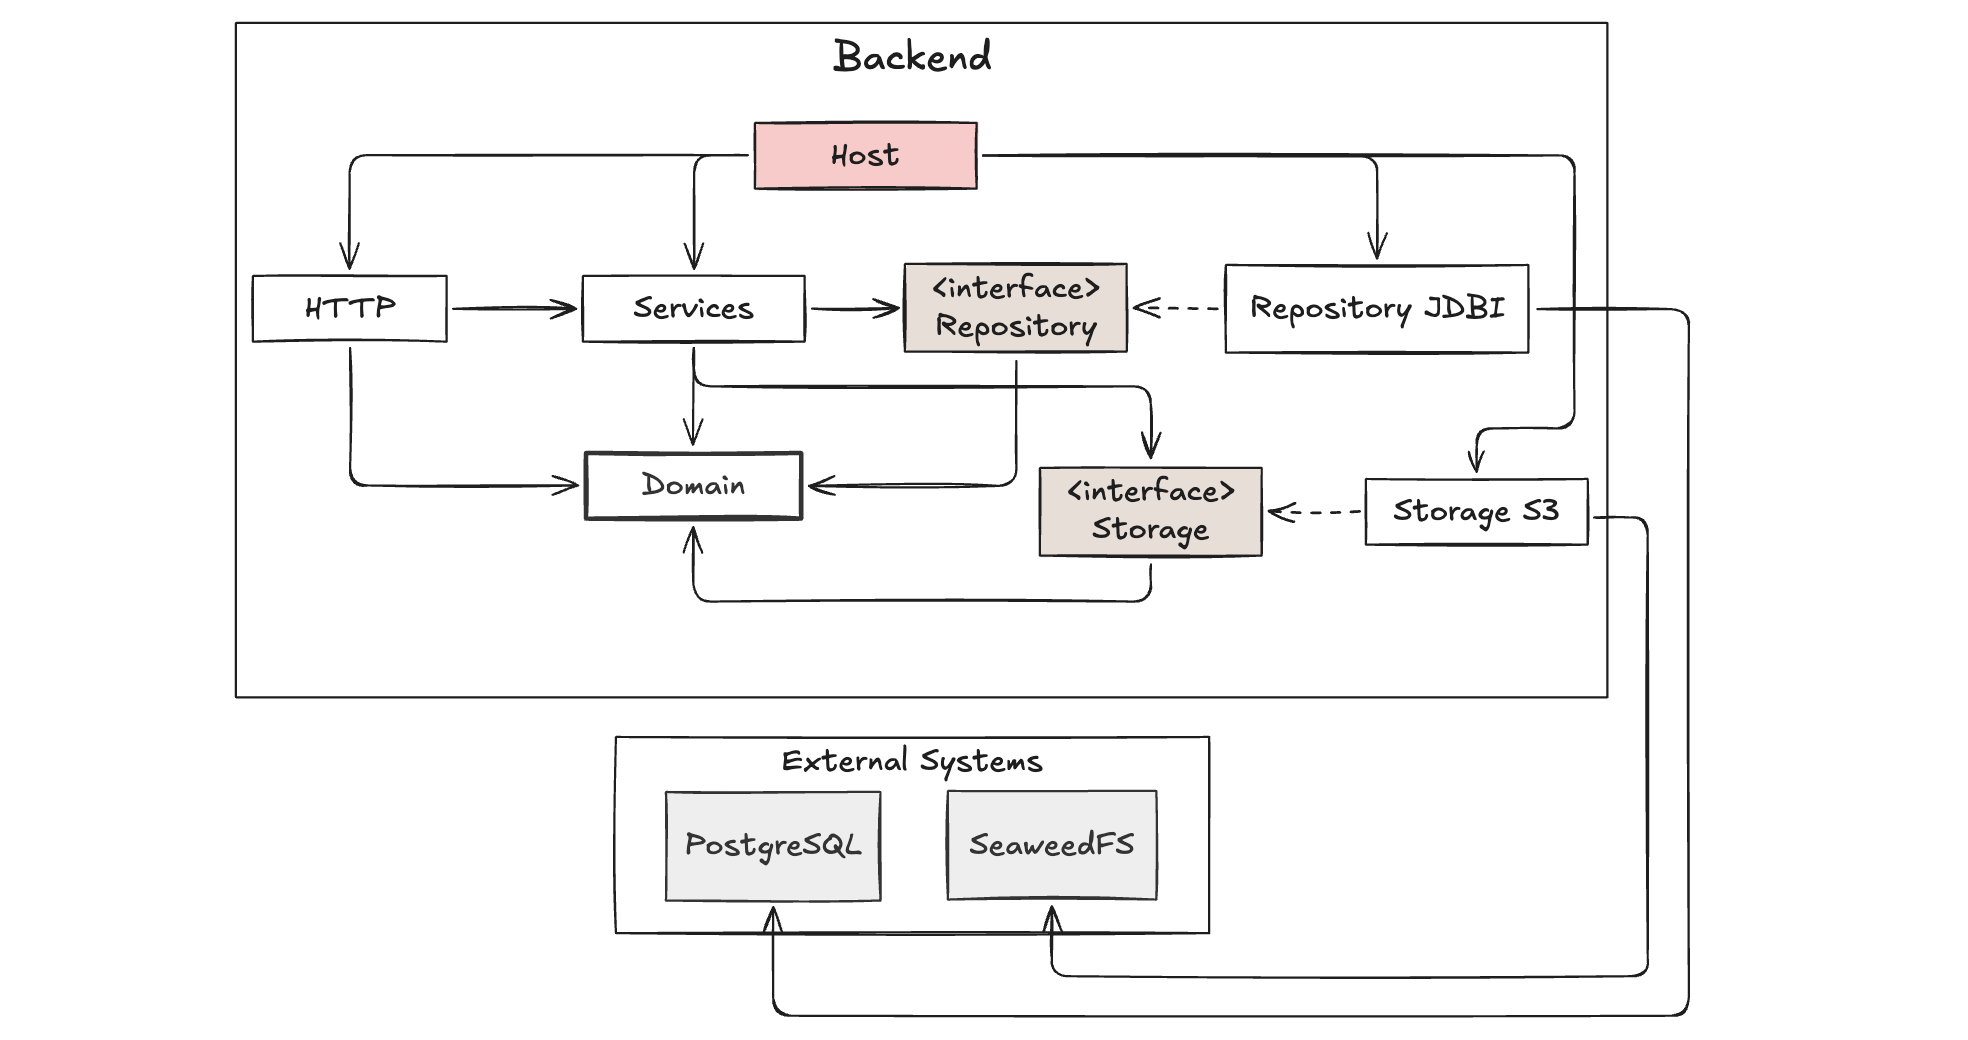
\includegraphics{./figures/backend_module_diagram.png}}
      \end{center}
      \caption{Backend module organization.}
      \label{fig:backend_layers}
\end{figure}

\begin{description}
      \item[HTTP] Defines the REST controllers that expose the API endpoints, each
            responsible for a bounded domain area (e.g., \texttt{ContentController},
            \texttt{UserController}, \texttt{CategoryController}). Also contains the
            authentication interceptor, argument resolvers, and Problem+JSON error handling.

      \item[Services] Contains the business logic, orchestrating operations across
            repositories and enforcing domain rules such as publication workflow transitions
            and permission checks.

      \item[Domain] Defines the core domain entities and value objects. This module
            has no dependencies on any other module, ensuring the domain model remains
            isolated from infrastructure concerns.

      \item[Repository] Defines the repository interfaces through which the service
            layer accesses persistent data. The concrete implementation, \texttt{Repository JDBI},
            implements these interfaces using JDBI, mapping SQL result sets to domain objects.
            This abstraction allows the persistence layer to be replaced without affecting
            business logic.

      \item[Storage] Defines the storage interface for multimedia files. The concrete
            implementation, \texttt{Storage S3}, integrates with SeaweedFS
            for binary file storage using the AWS S3 SDK~\cite{aws_s3_sdk}, as SeaweedFS
            exposes an S3-compatible API. An S3-compatible storage layer was chosen to
            avoid coupling the application to a specific storage provider while retaining a
            widely adopted interface. SeaweedFS was selected as a self-hosted
            implementation that satisfies the project's operational constraints and
            supports direct browser uploads, allowing large media files to bypass the
            application server during transfer. This approach reduces server load and keeps
            the backend responsible only for media metadata and access control.

      \item[Host] The root composition module, responsible for assembling the full
            application. It contains the Spring Boot entry point, all bean definitions, and
            the application configuration (database connection, storage credentials, server
            settings). No business logic resides here --- its sole purpose is wiring all
            modules together and bootstrapping the application.
\end{description}

The external systems used by the backend are \textbf{PostgreSQL}, accessed via the
JDBI repository implementation, and \textbf{SeaweedFS}, accessed via the S3 storage
implementation.

\section{Authentication} \label{sec:be_auth}

The authentication mechanism is described in Section~\ref{sec:arch_auth}. This
section covers the implementation details.

\subsection{JwtTokenGenerator} \label{sec:be_jwt}

Token generation and validation are handled by the \texttt{JwtTokenGenerator} class,
which encapsulates all JWT logic. Access tokens carry an HMAC-SHA256 message
authentication code (MAC), computed with a configurable secret key loaded at startup
via \texttt{JwtConfig}. The MAC key is initialised lazily and reused across requests. Refresh tokens are generated as
cryptographically random 32-byte strings encoded in Base64URL format using
\texttt{java.security.SecureRandom}.

\subsection{AuthenticationInterceptor} \label{sec:be_auth_interceptor}

The \texttt{AuthenticationInterceptor} implements Spring's \texttt{HandlerInterceptor}
interface, running before each request reaches a controller via the \texttt{preHandle}
method. It performs the following sequential checks:

\begin{enumerate}
      \item \textbf{Token extraction}: the interceptor reads the access token from the
            request cookies. If the endpoint requires authentication --- determined by the
            presence of a \texttt{@RequireRole} annotation or an \texttt{AuthenticatedUser}
            parameter --- and no valid token is found, the request is rejected with
            \texttt{401 Unauthorized}.

      \item \textbf{Role verification}: if the endpoint is annotated with
            \texttt{@RequireRole}, the role claim extracted from the JWT is compared against
            the required role without a database lookup. A mismatch results in a
            \texttt{403 Forbidden} response.
\end{enumerate}

If both checks pass, and the controller declares an \texttt{AuthenticatedUser}
parameter, the user is fetched from the database by the identifier in the JWT claims
and injected via \texttt{AuthenticatedUserArgumentResolver}. Endpoints that do not
declare this parameter incur no database lookup during authentication.

\section{Authorization} \label{sec:be_authorization}

Role-based access control (RBAC) is enforced at the HTTP layer via the
\texttt{@RequireRole} annotation. Each endpoint declares the minimum role required
to access it. The three roles --- \textit{Contributor}, \textit{Editor}, and
\textit{Administrator} --- form a strict permission hierarchy where each role inherits
all permissions of the roles below it, as described in
Section~\ref{sec:req_users}.

The adoption of a dedicated authorization library, such as Casbin~\cite{casbin}, was
considered as an alternative to enforcing the rules natively. General-purpose
authorization frameworks provide policy engines capable of expressing rich and
dynamic rule sets --- including attribute-based and relationship-based models --- and
are particularly valuable when access-control requirements are numerous, subject to
frequent change, or intended to be configurable at runtime without redeployment. In
the case of \textit{Diário LX}, however, the authorization model is deliberately small and
stable: it comprises three well-defined, hierarchically ordered roles whose
permissions are known at design time and are not expected to change. Under these
conditions, the expressive power of a policy engine offers limited practical benefit,
while introducing an additional external dependency, a separate policy definition to
maintain, and a layer of indirection between an endpoint and the rule that governs it.
Enforcing the rules natively through the \texttt{@RequireRole} annotation instead
keeps each endpoint's access requirement explicit and co-located with its declaration,
which favours readability and auditability. Adopting a library such as Casbin remains
a sensible evolution should the permission model grow in complexity --- for instance,
with per-resource ownership rules or finer-grained, runtime-configurable permissions
--- but for the current scope the additional complexity was not warranted.

\section{Error Handling} \label{sec:be_errors}

Error responses follow the \textbf{Problem Details for HTTP APIs} standard~\cite{rfc9457},
defined in RFC 9457. All error responses are returned with the
\texttt{application/problem+json} content type and contain the following fields:

\begin{itemize}
      \item \texttt{type} --- a URI identifying the problem type, pointing to the
            project's documentation at \texttt{github.com/jfmalencar/DiarioLX}.
      \item \texttt{title} --- a short, human-readable summary.
      \item \texttt{status} --- the HTTP status code.
      \item \texttt{detail} --- a human-readable explanation specific to the occurrence.
\end{itemize}

All problem instances are defined as static constants in the \texttt{Problem} class,
ensuring consistency across the codebase. Each problem carries a unique \texttt{type}
URI, a \texttt{title}, a \texttt{detail}, and an HTTP status code. Controllers invoke
\texttt{Problem.response()} to produce the appropriate \texttt{ResponseEntity} directly,
without relying on a centralised exception handler.

\section{Database Access} \label{sec:be_database}

Data access is handled through JDBI~\cite{jdbi}, a lightweight SQL convenience library
for the JVM. Unlike ORM-based approaches, JDBI provides direct control over SQL queries,
mapping result sets to domain objects explicitly. This choice favours simplicity and
transparency of database interactions over the abstraction overhead of a full ORM.

Database operations are executed within transactions managed by the
\texttt{TransactionManager} interface. Each call to \texttt{run\{\}} opens a JDBI
transaction, instantiates all repositories sharing the same database handle, and
ensures atomicity across multi-step operations. Rollback is handled automatically
by JDBI when an exception propagates.

\begin{lstlisting}[language=Java, caption={JdbiTransactionManager implementation.}]
@Named
class JdbiTransactionManager(
    private val jdbi: Jdbi,
    private val logger: Logger,
) : TransactionManager {
    override fun <R> run(block: (Transaction) -> R): R =
        jdbi.inTransaction<R, Exception> { handle ->
            val transaction = JdbiTransaction(handle, logger)
            block(transaction)
        }
}
\end{lstlisting}

\section{API Documentation} \label{sec:be_apidocs}

The API is documented using the OpenAPI standard~\cite{openapi}, generated
automatically by \texttt{springdoc-openapi}~\cite{springdoc} and served via
Scalar~\cite{scalar}, a modern API reference UI. Custom annotations
(\texttt{@MayReturnNotFound}, \texttt{@MayReturnBadRequest}, etc.) were defined
to reduce boilerplate in controller declarations while maintaining accurate schema
documentation. The documentation is available at \texttt{/docs} when the
application is running.

\section{Tests} \label{sec:be_tests}

Testing is organized by module, with dedicated test suites for the repository,
service, and HTTP layers. At the current beta stage, the test suites are in an
early phase and do not yet provide full coverage.

The backend test suite is integrated into the project's continuous integration
pipeline via GitHub Actions, running automatically on every push.

\subsection{Unit Tests} \label{sec:tests_be_unit}

Unit tests cover the repository and service layers in isolation. Repository tests
validate SQL queries and result set mappings against a dedicated test database
instance. Service tests validate business logic, including publication workflow
state transitions and permission checks, independently of the HTTP and persistence
layers.

\subsection{Integration Tests} \label{sec:tests_be_integration}

Integration tests validate the full request-response cycle of the API, exercising
the HTTP, service, and repository layers together.